\documentclass[tikz,border=5pt]{standalone}
% Shared visual grammar: role fills, dark connectors, and 7-point typography.
% Build each standalone figure from this directory. No external images required.
\pdfinfoomitdate=1
\pdftrailerid{}
\usepackage[T1]{fontenc}
\usepackage{helvet}
\renewcommand{\familydefault}{\sfdefault}
\usepackage{amsmath,amssymb}
\hyphenpenalty=10000
\exhyphenpenalty=10000
\usetikzlibrary{arrows.meta,calc,fit,positioning,decorations.pathreplacing,backgrounds}
\definecolor{ink}{HTML}{172B3A}
\definecolor{muted}{HTML}{586D85}
\definecolor{datafill}{HTML}{F1F5F9}
\definecolor{dataline}{HTML}{62748E}
\definecolor{modelfill}{HTML}{E5E9FF}
\definecolor{modelline}{HTML}{7887C7}
\definecolor{llmfill}{HTML}{FFE4E8}
\definecolor{llmline}{HTML}{E68494}
\definecolor{truthfill}{HTML}{D0FAE5}
\definecolor{truthline}{HTML}{35A782}
\newcommand{\seven}{\fontsize{7}{8.5}\selectfont}
\tikzset{
 every node/.append style={font=\seven,text=ink,align=center},
 box/.style={draw=dataline,fill=white,rounded corners=3pt,line width=.65pt,inner sep=5pt,minimum height=8mm},
 data/.style={box,fill=datafill},
 model/.style={box,draw=modelline,fill=modelfill},
 llm/.style={box,draw=llmline,fill=llmfill},
 truth/.style={box,draw=truthline,fill=truthfill},
 title/.style={font=\seven\bfseries,inner sep=1pt},
 word/.style={text=muted,inner sep=1pt,align=center},
 label/.style={fill=white,inner xsep=2pt,inner ysep=1pt,text=muted},
 flow/.style={-{Stealth[length=2.4mm,width=1.9mm]},draw=ink,line width=1.2pt,shorten >=1.5pt},
 branch/.style={-{Stealth[length=2mm,width=1.6mm]},draw=ink,line width=.9pt,shorten >=1pt},
 route/.style={draw=ink,line width=1.2pt},
 update/.style={-{Stealth[length=2.2mm,width=1.7mm]},draw=modelline,line width=1pt,dash pattern=on 3pt off 2pt,shorten >=1.5pt},
 boundary/.style={draw=dataline,dash pattern=on 3pt off 2pt,rounded corners=3pt,line width=.6pt},
 chip/.style={minimum height=4mm,inner xsep=3pt,inner ysep=1.5pt,rounded corners=2pt},
}
% Optional role key. Anchor at the center of an uncluttered final row.
\newcommand{\rolekey}[2]{
 \node[word,anchor=east] at (#1-6.6,#2) {\textit{Key}};
 \node[data,chip] at (#1-5.2,#2) {records / data};
 \node[model,chip] at (#1-1.9,#2) {learned model / policy};
 \node[llm,chip] at (#1+1.65,#2) {LLM signal};
 \node[truth,chip] at (#1+4.95,#2) {labels / evaluation};
}

\newcommand{\comparisonfont}{\fontsize{9}{11}\selectfont}
\begin{document}
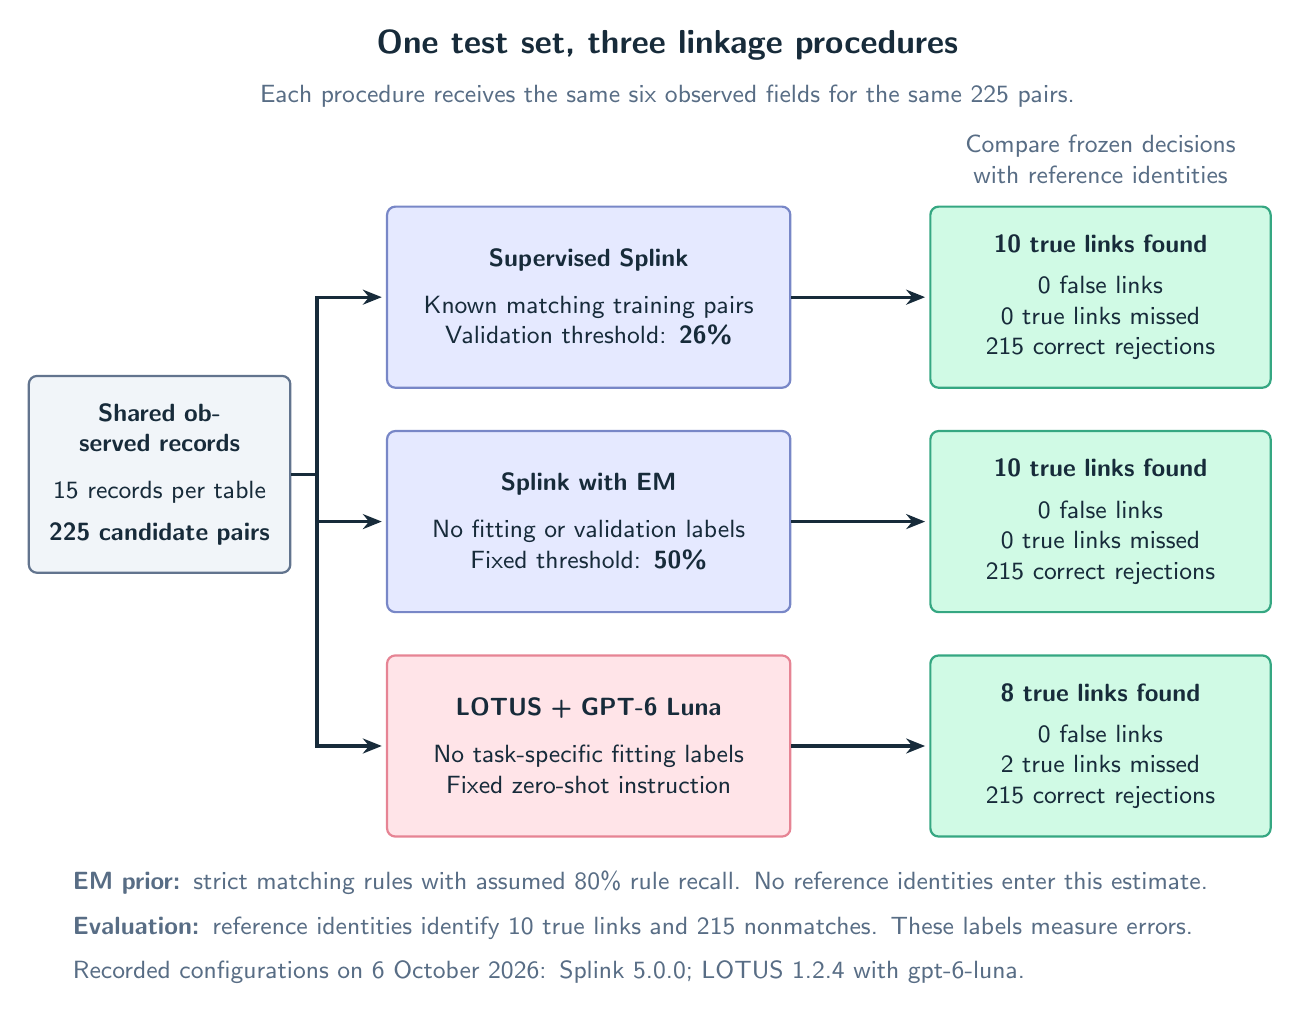
\begin{tikzpicture}[every node/.append style={font=\comparisonfont},
  box/.append style={inner sep=6pt,line width=.8pt}]

\node[title,font=\fontsize{12}{14}\selectfont\bfseries] at (8,0) {One test set, three linkage procedures};
\node[word] at (8,-.65) {Each procedure receives the same six observed fields for the same 225 pairs.};
\node[word,text width=42mm] at (13.5,-1.45) {Compare frozen decisions\\with reference identities};

\node[data,text width=29mm,minimum height=25mm] (pairs) at (1.55,-5.45) {
  \textbf{Shared observed records}\\[6pt]
  15 records per table\\[4pt]
  \textbf{225 candidate pairs}};
\node[model,text width=47mm,minimum height=23mm] (supervised) at (7,-3.2) {
  \textbf{Supervised Splink}\\[6pt]
  Known matching training pairs\\
  Validation threshold: \textbf{26\%}};
\node[model,text width=47mm,minimum height=23mm] (em) at (7,-6.05) {
  \textbf{Splink with EM}\\[6pt]
  No fitting or validation labels\\
  Fixed threshold: \textbf{50\%}};
\node[llm,text width=47mm,minimum height=23mm] (lotus) at (7,-8.9) {
  \textbf{LOTUS + GPT-6 Luna}\\[6pt]
  No task-specific fitting labels\\
  Fixed zero-shot instruction};

\node[truth,text width=39mm,minimum height=23mm] (sout) at (13.5,-3.2) {
  \textbf{10 true links found}\\[4pt]
  0 false links\\
  0 true links missed\\
  215 correct rejections};
\node[truth,text width=39mm,minimum height=23mm] (eout) at (13.5,-6.05) {
  \textbf{10 true links found}\\[4pt]
  0 false links\\
  0 true links missed\\
  215 correct rejections};
\node[truth,text width=39mm,minimum height=23mm] (lout) at (13.5,-8.9) {
  \textbf{8 true links found}\\[4pt]
  0 false links\\
  2 true links missed\\
  215 correct rejections};

\draw[route] (pairs.east) -- (3.55,-5.45);
\draw[flow] (3.55,-5.45) |- (supervised.west);
\draw[flow] (3.55,-5.45) |- (em.west);
\draw[flow] (3.55,-5.45) |- (lotus.west);
\draw[flow] (supervised) -- (sout);
\draw[flow] (em) -- (eout);
\draw[flow] (lotus) -- (lout);

\node[word,text width=151mm,align=left] at (8,-11.2) {
  \textbf{EM prior:} strict matching rules with assumed 80\% rule recall. No reference identities enter this estimate.\\[5pt]
  \textbf{Evaluation:} reference identities identify 10 true links and 215 nonmatches. These labels measure errors.\\[5pt]
  Recorded configurations on 6 October 2026: Splink 5.0.0; LOTUS 1.2.4 with gpt-6-luna.};

\end{tikzpicture}
\end{document}
